\hsection{Basics of Classes}%
%
We learned about simple datatypes in \cref{sec:simplyDataTypesAndOperations} and about collections in \cref{sec:collections}.
However, in many situations, we deal with data that cannot satisfyingly represented by either of them alone.
Often, datatypes and the operations on them form a semantic unit.

Imagine, for example, you would like to implement mathematical operations for complex numbers.\footnote{%
\python\ already offers the datatype \pythonilIdx{complex}, but for the sake of the example, assume it does not.}
Of course, you could represent complex numbers as \pythonil{tuple[float, float]}, but this comes with several drawbacks.
On one hand, not \emph{every} tuple of two \pythonils{float} is to be understood as a complex number.
So just from the \pgls{signature} of your functions, i.e., just based on its parameters and return types, it is not immediately clear that your functions are for complex numbers.
All we can directly see is that they are for tuples of two \pythonils{float}.
On the other hand, the two parts of a complex numbers, the real part and the imaginary part, have two distinct and different meanings.
It would not immediately be clear whether the first number of the tuple is the real or the imaginary part.
Indeed, we could also represent complex numbers in polar form, in which case the two tuple elements would have yet different meanings.
Also, the standard textual representation of tuples of two \pythonils{float} would be something like~\pythonil{"(3.0, 4.0)"}, whereas we would probably prefer something like~\pythonil{"3+4i"}.

The first important use-cases of \pythoniles{class} in \python\ is that they offer us a way to define a data structure together with the operations for it as one semantic unit.
This allows us to define a \pythonil{class} for complex numbers which has attributes with the name \pythonil{real_part} and \pythonil{imaginary_part}.
We can define operators that work with instances of this \pythonil{class}, making it immediately clear how and when they are to be used-
And this \pythonil{class} can then have default textual representations of our liking.

A second situation where ability to define functions and we have learned so far hits a limit arises with \pglspl{API}.
Let us be ambitious and imagine that you wanted to create a versatile system that can produce documents.
On the output side, you want to support different formats, say LibreOffice~\cite{DF2024LTDF,GL2012LTSOOSSCBAFACSOL}, Microsoft~Word~\cite{MS2024MW,DR2019STFAWAUMW}, and Adobe~PDF~\cite{A2024WDPM,A2008P3DMPDFP1P1}.
On the input side, you would like to provide the user with a uniform way to create documents, to add text paragraphs, to insert graphics, to set the font of texts, and so on.
This input side \pgls{API} should be the same for all output formats.
It would not just consist of a single function, but several groups of functions.
There could even be nested hierarchies of operations that you would like to support, e.g., the ability to divide a text into chapters which can be divided into paragraphs which can be divided into runs of text with different fonts.
Obviously, these operations will be implemented differently for the different output formats.
We could try to solve this by making different modules with functions of the same \pglspl{signature} for the different output formats.
But this would be a huge hassle, in particular since there would be no way to define a central blueprint of \inQuotes{how the \pgls{API} looks like.}
It can easily lead to inconsistencies during the software life cycle.
If we slightly change the \pgls{signature} of one function, we need to implement this in all of the modules.
There also is no way that a tool like \ruff\ could tell is if some module is no longer synchronized due to the lack of a central blueprint.

Classes offer us the necessary abstraction:
We could specify a base class \pythonil{Document} for document objects that provides methods for the necessary operations, from adding text to aligning figures.
These operations could just \pythonilIdx{raise} a \pythonilIdx{NotImplementedError}.
Then, for each output format, we could derive a new subclass from this base class with the actual implementation of the methods.
The code on the user side could treat all these different document types the same, because all of them would be instances of \pythonil{Document} with the same operations.
The implementation-specific stuff would all be invisible to the user, exactly as it should be.
So the second important use case for classes are that they offer us a very nice abstraction for defining and implementing \pglspl{API}.

Classes therefore can solve two important problems where the basic datatypes and plain functions we learned about are not sufficient:
First, they allow us to semantically and clearly group data and operations together.
Second, they offer us a simple way to group several operators under one \pgls{API}, which then -- transparently to the user -- can be implemented in different ways.
In this chapter, we discuss \pythoniles{class} in \python.
Syntactly, \pythoniles{classes} follow the general blueprint below:%
%
\begin{pythonSyntax}
class MyClass:   # or `class MyClass(MyBaseClass)`
    """Docstring of the class."""

    def __init__(self) -> None:
        """Docstring of the initializer __init__."""
        # initialize all attributes
        #: Meaning of attribute 1
        self.attribute_1: type hint = initial value
        # ...

    def my_method(self, param1, param2) -> result:
        """Docstring of my_method."""
        # compute something using the attributes
\end{pythonSyntax}
%
\bestPractice{className}{\sloppy%
Class names should follow the CapWords convention (often also called camel case), i.e., look like \pythonil{MyClass} or \pythonil{UniversityDepartment} (not \pythonil{my_class} or \pythonil{university_department})~\cite{PEP8}.}%
%
\hsection{A Simple Immutable Class for Points in the Two-Dimensional Euclidean Plane}%
\label{sec:immutableClassPoints2D}%
%
\gitPython{\programmingWithPythonCodeRepo}{classes/point.py}{--args format}{classes:point}{%
A class for representing points in the two-dimensional Euclidean plane.}%
%
\gitPythonAndOutput{\programmingWithPythonCodeRepo}{classes}{point_user.py}{--args format}{classes:point_user}{%
An example of using our new \pythonil{class Point} from \cref{lst:classes:point}.}%
%
We begin directly with an example.
Assume that we want to write a program that processes points in the two-dimensional Euclidean plane.
Every point is defined by its x\nobreakdashes~and y\nobreakdashes-coordinate.
We could use a \pythonil{tuple} of two numbers, say a~\pythonil{tuple[int | float, int | float]}, to represent such points.
This is totally fine and a quick solution.

However, this solution lacks semantics, i.e., it lacks a clear and obvious meaning.
There is nothing that says that a \pythonil{tuple[int | float, int | float]} must be a point in the two-dimensional Euclidean plane.
It could just as well be a tuple of travel time and an associated cost for a train ride from Hefei to Beijing, taken from the train schedule of a particular day.
Basically, it just is a grouping of two numbers.
The same lack of semantics appears when we try to implement operations that process our points.
A function that computes the distance between two such points would just take two \pythonils{tuple} as input.
Of course, I should pass in only \pythonils{tuple} that actually represent points in the two-dimensional plane.
But nothing really can stop me from passing in other tuples, such as \pythonils{tuple} holding the travel times and associated costs for train rides from Hefei to Beijing.
Of course, the results would probably not make any sense.
Yet, such situations may arise from misunderstandings or lack of documentation.

In the ideal case, if I am working with points in the two-dimensional Euclidean plane, then I have a data structure that clearly and unambiguously is designed for such points and such points only.
The operations for the points should only accept instances of this data structure as input (and raise\pythonIdx{raise} exceptions\pythonIdx{Exception} if fed something else as arguments).
If I am accessing the x\nobreakdashes-coordinate of a point, it should be absolutely clear from the semantics and names involved that this is, indeed, the x\nobreakdashes-coordinate and not something else, not just the first number of a \pythonil{tuple} of two numbers.

Such clear semantics can be achieved with \pythoniles{class}\pythonIdx{class} in \python.
In \cref{lst:classes:point}, you can find exactly this example.
We create the \pythonil{class Point}\pythonIdx{class} inside a \python\ file \textil{point.py}.
This is done relatively easily:
All we have to do is to begin a block with, well, \pythonil{class Point:}.
Inside this block, we will place all the \emph{methods} of the \pythonilIdx{class}.
Methods are like functions, but their first parameter is always called \pythonilIdx{self} and always is an instance of the class, i.e., an object.
Either way, all these methods go into the class block.
Of course, first, we always place a \pgls{docstring}.%
%
\bestPractice{classDocString}{%
At the beginning of a \pythonilIdx{class}, a \pgls{docstring} is placed which describes what the class is good for. %
This \pgls{docstring} and include \pglspl{doctest} to demonstrate the class usage, or such \pglspl{doctest} can be placed in the \pgls{docstring} of the module.%
}%
%
Our class \pythonil{Point} will have two attributes, \pythonil{x} and~\pythonil{y}.
A attribute is a variable that every single instance of the class has.
We later want to be able to create one instance of \pythonil{Point} with the x\nobreakdashes-coordinate~5 and the y\nobreakdashes-coordinate~10 and then another instance with the x\nobreakdashes-coordinate~2 and the y\nobreakdashes-coordinate~7.
So each instance of \pythonil{Point} needs to have these two attributes.

Therefore, \pythonil{Point} needs a initializer, i.e., a special method that creates and initializes these attributes.
This method is called~\dunder{init}.
As said, every method of a class must have a parameter~\pythonilIdx{self}, which is the instance of the class (the object) upon which the method is called.
The initializer \dunder{init} is a special method, so it also has this parameter~\pythonilIdx{self}.
Additionally, we demand that two parameters~\pythonil{x} and~\pythonil{y} be passed in when we create an instance of~\pythonil{Point}.
We allow the values to be either \pythonils{int} or \pythonils{float}.

Inside every method of a class, the attributes of objects are accessed via the parameter~\pythonilIdx{self}.
We can read the attribute~\pythonil{x} of an object inside a method of the class by writing~\pythonil{self.x}.
Here, \pythonil{self.x} can be used just like a normal local variable.
We can store the value~\pythonil{a} in a (mutable) attribute~\pythonil{x} of the current object in a method of the class by writing~\pythonil{self.x = a}.
This value will then remain the same until it is changed, even after the execution of the method is completed.%
%
\bestPractice{attributes}{%
Object attributes must only be created inside the initializer~\dunder{init}. %
An initial value must immediately be assigned to each attribute.%
}
%
We only want to allow \pythonils{Point} that have finite coordinates.
As explained in the \cref{sec:exceptions} on \pythonilsIdx{Exception}, it is better to immediately signal errors if we encounter invalid data.
So we want to sort out non-finite coordinates right when someone attempts to create the \pythonil{Point} object.
Thus, the first thing we do in the initializer is to use the \pythonilIdx{isfinite} function from the \pythonilIdx{math} module.
If either \pythonil{x} or \pythonil{y} is not finite, then we raise\pythonIdx{raise} a \pythonilIdx{ValueError}.
Otherwise, we set \pythonil{self.x: Final[int | float] = x} and \pythonil{self.y: Final[int | float] = y}.\footnote{%
Strictly speaking, it could also make sense to check whether \pythonil{x} and \pythonil{y} are indeed either \pythonil{int} or \pythonil{float}. %
For example, we could check if \pythonil{isinstance(x, int | float)}\pythonIdx{isinstance} and this is \pythonil{False}, raise\pythonIdx{raise} a~\pythonilIdx{TypeError}. %
However, that would make the example overly long, so I am not doing this here.%
}
These lines create the attributes \pythonil{self.x} and \pythonil{self.y} of the object which was passed in via the parameter~\pythonil{self}.
Additionally, the \pgls{typeHint} \pythonilIdx{Final} from the \pythonilIdx{typing} module annotates a variable as immutable~\cite{PEP591}.
In other words, we do not allow the coordinates of our \pythonils{Point} to change after object creation.%
%
\bestPractice{attributeTypeHint}{%
Every attribute of an object must be annotated with a \pgls{typeHint} and a documentation comment when created in the initializer~\dunder{init}~\cite{LM2024WTMD}. %
\pglspl{typeHint} work as with normal variables.}%
%
\bestPractice{attributeFinal}{%
The \pgls{typeHint} \pythonilIdx{Final}\pythonIdx{typing!Final} marks an attribute as immutable. %
All attributes that you do not intend to change should be annotated with~\pythonilIdx{Final}\pythonIdx{typing!Final}.%
}%
%
\bestPractice{attributeDocstring}{%
An attribute is documented in the line \emph{above} the attribute initialization by writing a \emph{comment} starting with \pythonilIdx{\#: }, which explains the meaning of the attribute~\cite{SD2024DCAD}. %
(Sometimes, the documentation is given as string directly below the attribute definition~\cite{PEP287}, but we stick to the former method, because it has proper tool support, e.g., by~\sphinx.)%
}%
%
After properly defining our initializer, we can now do something like~\pythonil{p = Point(1, 2)}.
This creates a new object as an instance of our \pythonilIdx{class} \pythonil{Point}.
Therefore, first, the necessary memory is allocated.
Then, the initializer is invoked as~\pythonil{\_\_init\_\_(p, 1, 2)}.
As a result, \pythonil{p} now refers to a \pythonil{Point}~object.
The attribute \pythonil{p.x} has the value~\pythonil{1} and \pythonil{p.y} has value~\pythonil{2}.

From the knowledge that \pythonil{p} is an instance of \pythonil{Point}, we can immediately see that \pythonil{p.x} and \pythonil{p.y} are its x-\ and y\nobreakdashes-coordinate, respectively.
There is no way to mistake the meaning of these variables.
Of course, our \pglspl{docstring} with \pglspl{doctest} and \pglspl{typeHint} further help the reader to understand their meaning.

Having a new class for points in the two-dimensional plane is already nice.
But \pythoniles{class} also allow us to define operations on such points in form of methods.
As an example, we implement a method \pythonil{distance} that computes the distance between two points.
You would have a point~\pythonil{p1} and invoke \pythonil{p1.distance(p2)} to compute the distance to another point~\pythonil{p2}.
The computation itself will follow \cref{eq:euclideanDistance} from our recent endeavor to operations on iterations in \cref{sec:operationsOnIterators}.
We therefore need to import the \pythonilIdx{sqrt} function from the \pythonilIdx{math} module.

Our new method \pythonil{distance} will have two parameters, \pythonilIdx{self}, which will be the object upon which we invoke the method~(\pythonil{p1}~in the above example) and~\pythonil{p}, the other object~(or \pythonil{p2} above).
It then just has to compute the Euclidean distance~\pythonil{sqrt((self.x - p.x) ** 2 + (self.y - p.y) ** 2)}.
Inside a method of an object, \pythonilIdx{self} always refers to the object itself.
Therefore, \pythonil{self.x}~is the x\nobreakdashes-coordinate of the current object and \pythonil{self.y}~is its~y\nobreakdashes-coordinate.
\pythonil{p.x}~is the x\nobreakdashes-coordinate of the point~\pythonil{p} that was passed in as actual parameter of the method, and \pythonil{p.y}~is its y\nobreakdashes-coordinate.
Notice that the \pgls{docstring} not just explains how this method is used, but also provides a simple example in form of a~\pgls{doctest}.
If you compute \pythonil{Point(1, 1).distance(Point(4, 4))}, then the expected result is something like~4.243.%
%
\begin{sloppypar}%
In this \pgls{doctest} -- \pythonil{Point(1, 1).distance(Point(4, 4))} -- we only provided a single parameter to the method~\pythonil{distance}.
When calling the method~\pythonil{distance}, we never need to provide a value of the parameter~\pythonilIdx{self} directly.
Instead, it will be provided indirectly:
If we have two points~\pythonil{p1} and~\pythonil{p2} and invoke~\pythonil{p1.distance(p2)}, then~\pythonil{self = p1} will be set automatically.
Hence, even though we declared our method as~\pythonil{def distance(self, p: "Point") -> float}, which looks as if we need to provide two parameters~(\pythonilIdx{self} and~\pythonil{p}), we only need to provide one, namely~\pythonil{p}.%
\end{sloppypar}%
%
Reading this again, we notice that the parameter~\pythonil{p} is annotated with a very strange \pgls{typeHint}:
One would expect that we would annotate it with~\pythonil{Point}, instead it is annotated with the string~\pythonil{"Point"}.
This has the simple reason that the complete class \pythonil{Point} is only defined \emph{after}, well, the complete definition of class~\pythonil{Point} and, therefore, not yet available as type \emph{inside} its definition.
Using the string here is therefore just a crutch with no real other effect.
%
%
\bestPractice{methodDocstring}{%
All methods of \pythoniles{class} must be annotated with \pglspl{docstring} and \pglspl{typeHint}.%
}%
\bestPractice{ownClassTypeHint}{%
When using a class~\pythonil{C} as \pgls{typeHint} \emph{inside} the definition of the class~\pythonil{C}, you must write~\pythonil{"C"} instead of~\pythonil{C}. %
(Otherwise, static code analysis tools and the \python\ interpreter get confused.)%
}%
%
We could now go on and add more methods that do reasonable computations with instances of~\pythonil{Point}.
For now, this simple example will suffice.
Let us instead take a look on how one would use our new class.

In \cref{lst:classes:point_user}, we begin by creating one instance of~\pythonil{Point} and store it in a variable~\pythonil{p1}.
Since~\pythonil{p1} is supposed to reference an instance of~\pythonil{Point}, its \pgls{typeHint} should denote this.
Here we can use \pythonil{Point} just like any other datatype.
We write \pythonil{p1: Point = Point(3, 5)}.
The resulting new instance of \pythonil{Point} should have its attribute~\pythonil{x} set to~\pythonil{3} and its attribute~\pythonil{y} set to~\pythonil{5}.
We can access them via~\pythonil{p1.x} and~\pythonil{p1.y}.
Of course we can also use them in an \pgls{fstring}.

We can check if an object~\pythonil{o} is an instance of our class \pythonil{Point} by writing~\pythonil{isinstance(o, Point)}.
For \pythonil{p1}, this returns~\pythonil{True}.

We now create a second instance, \pythonil{p2}, of the class \pythonil{Point}.
We assign \pythonil{7} to \pythonil{p2.x} and \pythonil{8} to \pythonil{p2.y} via the \dunder{init} initializer, which is automatically invoked when we write~\pythonil{Point(7, 8)}.
We can again print the values of these attributes using an \pgls{fstring}.
While \pythonil{isinstance(p2, Point)} is again \pythonil{True}, \pythonil{isinstance(5, Point)} returns \pythonil{False}.

While being instances of the same class, \pythonil{p1} and \pythonil{p2} are different objects.
Therefore, \pythonil{p1 is p2} yields~\pythonil{False}.%
%
\begin{sloppypar}%
We can now also use our method \pythonil{distance}.
\pythonil{p1.distance(p2)}, i.e., the distance from~\pythonil{p1} to~\pythonil{p2}, is the same as \pythonil{p2.distance(p1)}, i.e., the distance from~\pythonil{p2} to~\pythonil{p1}.
Both are equal to~5, because~$\sqrt{(7 - 3)^2+ (8 - 5)^2}=\sqrt{4^2 + 3^2}=\sqrt{25}=5$.%
\end{sloppypar}%
%
\pythonil{Point} can indeed be used like any other datatype that we discussed before.
For example, we can have lists of instances of \pythonil{Point}~(and the appropriate \pgls{typeHint} would then by \pythonil{list[Point]}).
We can even create such a list with list comprehension\pythonIdx{list!comprehension}\pythonIdx{comprehension!list}, exactly as we learned back in \cref{sec:listComprehension}.
And we can then process this list by writing a generator expression which transforms the points to strings, just as we discussed in \cref{sec:generatorExpressions}.
The expression generates a sequence of strings of the form \textil{"(x, y)"}, which are then concatenated by the \pythonilIdx{join}\pythonIdx{str!join} method of the string~\pythonil{", "}~(see \cref{sec:loopsOverSequences}).
The result can be seen at the bottom of \cref{exec:classes:point_user}.

The objects of our \pythonil{Point} class are \emph{immutable}, i.e., once created, the attributes cannot be changed anymore.\footnote{%
Well, in \python, \pglspl{typeHint} are just hints and not enforced by the interpreter~\cite{PEP591}. %
So the x\nobreakdashes-~and y\nobreakdashes-attributes of instances of \pythonil{Point} can actually be changed. %
However, tools like \mypy\ will detect such mistakes and report them~\cite{PEP591}.%
}
The x\nobreakdashes-~and y\nobreakdashes-attributes are initialized by the \pythonil{\_\_init\_\_} initializer.
They are marked with the \pgls{typeHint} \pythonilIdx{Final} and thus changing them is an error.
In many cases, making objects immutable is a good design pattern.%
%
\quotation{B2008EJ}{%
Classes should be immutable unless there’s a very good reason to make them mutable{\dots}.
If a class cannot be made immutable, limit its mutability as much as possible.%
}%
%
\begin{definition}[Immutable]%
After their creation, the attributes of \emph{immutable} objects cannot be modified anymore.%
\end{definition}%
%
Creating classes whose instances are immutable has several benefits:
Code gets easier to understand, because we do not need to think about whether, when, or how an object changes (because it cannot).
The elements of sets and the keys of dictionaries in \python, for example, must be immutable objects because they store objects based on their hash codes which, in turn, are based on the attributes of these objects.
If the attributes would change, so would the hash codes, which means that the objects could no longer be found.
This is particularly useful in parallel programming, where mutable shared state could lead to complex bugs and race conditions.

Still, there also are many cases where we want to create objects whose attributes can change.
We will explore one of them in the next section.%
\FloatBarrier%
\endhsection%
%
\hsection{Encapsulation and Accurately Adding Floating Point Numbers}%
\FloatBarrier%
%
We now want to implement our first maybe actually useful piece of code, something that can be used in a real productive system.\footnote{%
Yes, we did implement the method of LIU Hui~(\zhb{刘徽}) for approximating~\numberPi\ and Heron's Method for approximating the square root. %
These implementations were not more accurate than the constant and function \python\ already has built in. %
But they are nice, though, I did enjoy doing them.}
To do such a cool thing, let us first revisit the limitations of the datatype \pythonil{float} from way back in \cref{sec:float}. %
%
\begin{figure}%
\centering%
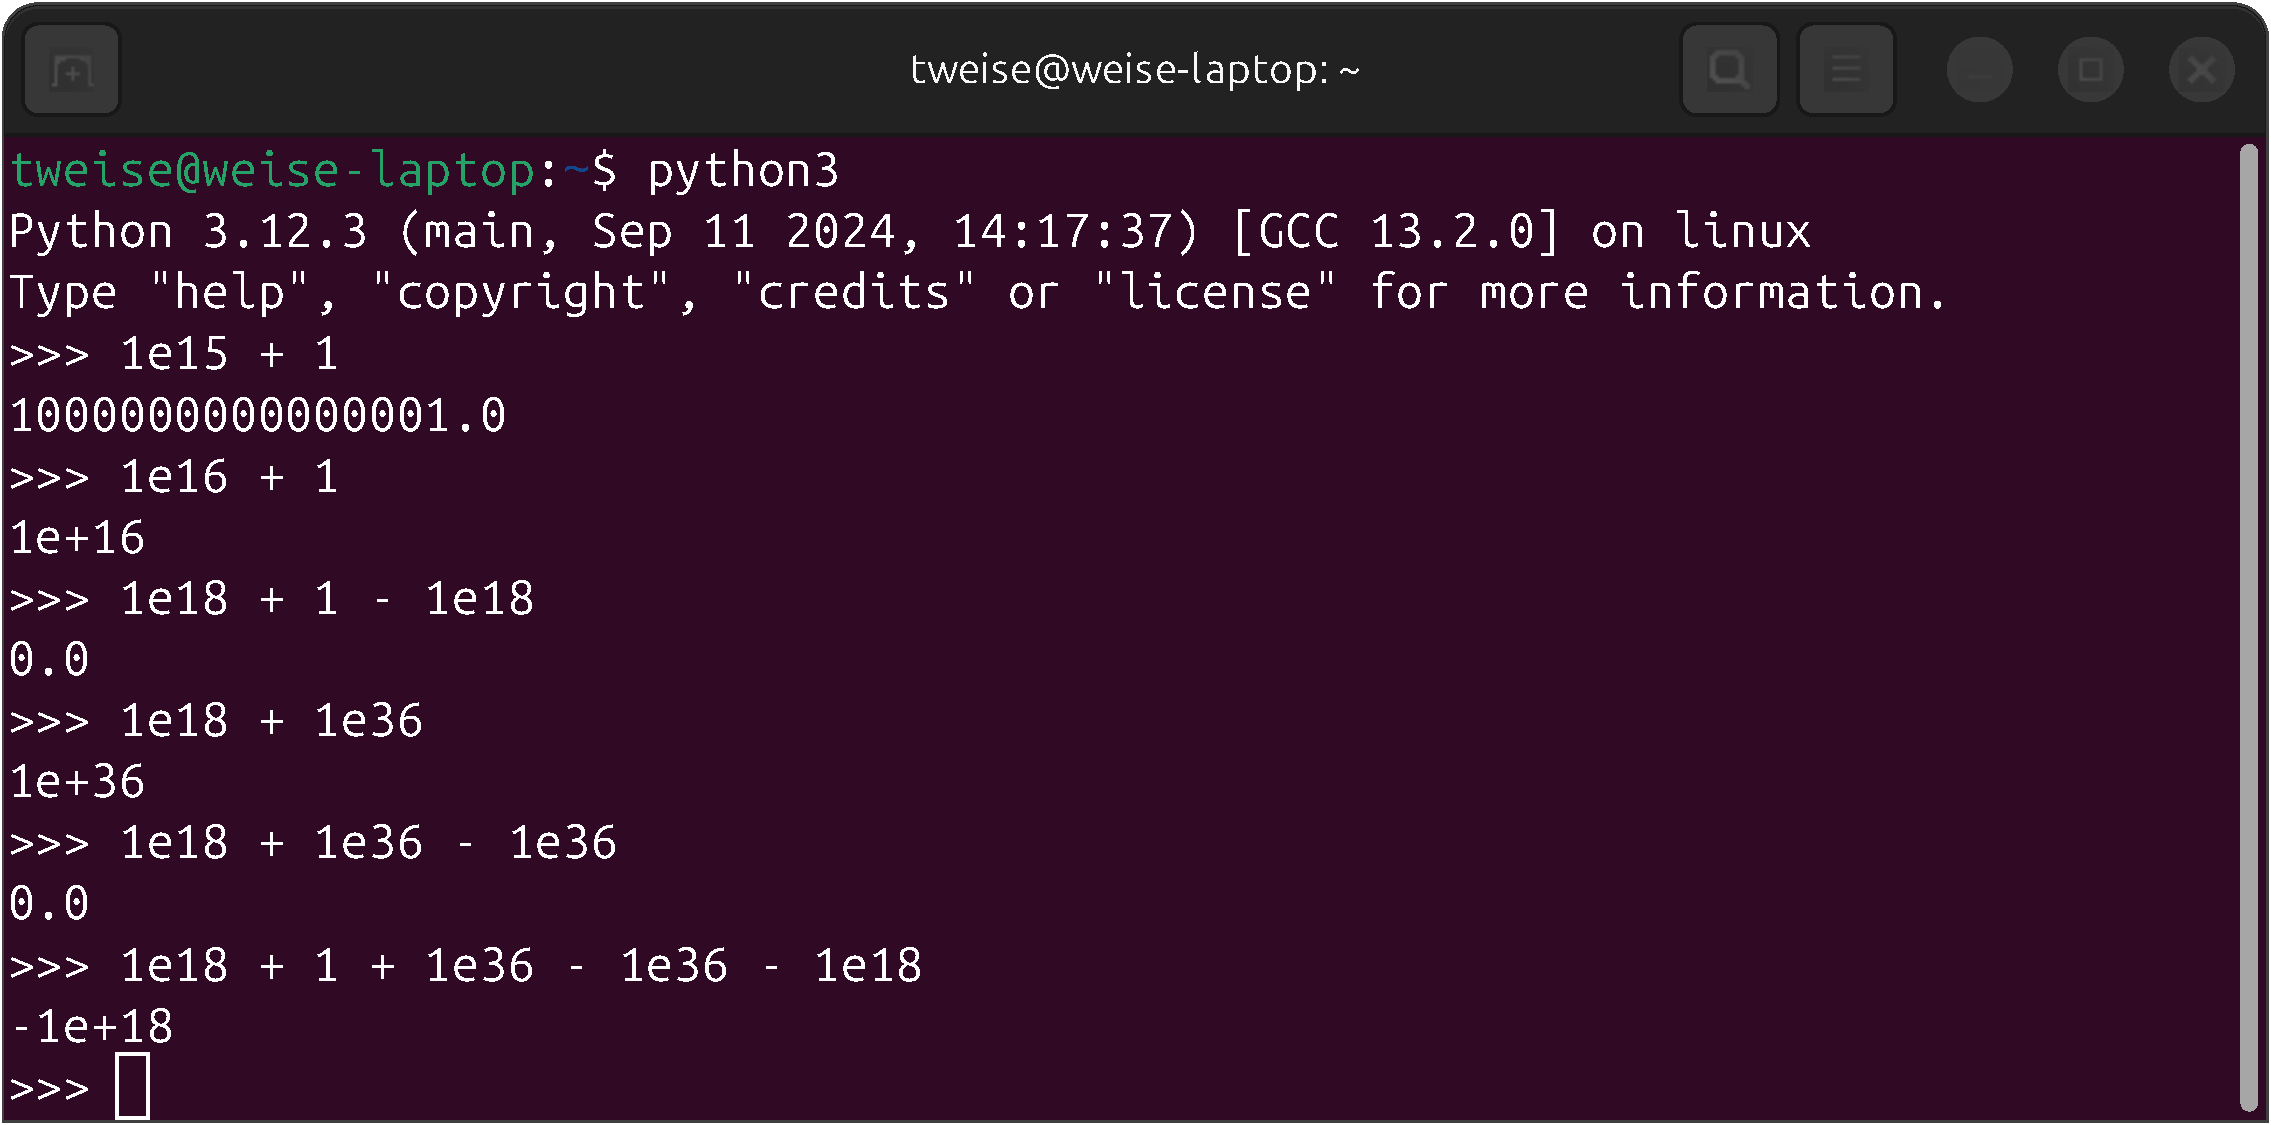
\includegraphics[width=0.7\linewidth]{\currentDir/addingFloatsError}%
\caption{Errors occurring when adding floating point numbers due to the limited precision of the datatype~\pythonilIdx{float}.}%
\label{fig:addingFloatsError}%
\end{figure}%
%
We learned that the datatype \pythonilIdx{float} can represent numbers accurately to about fifteen to sixteen digits.
This is illustrated in \cref{fig:addingFloatsError}:
If we add~\pythonil{1} to~$10^{15}=\pythonil{1e15}$, the correct result is~\pythonil{1000000000000001.0}.
However, if we add~\pythonil{1} to~$10^{16}=\pythonil{1e16}$, the result is still~\pythonil{1e16}.
It is not possible to represent the number~$1+10^{16}$ correctly with the 64~bit double precision floating point numbers that \python\ offers~\cite{PSF2024FPAIAL}.
Usually, that itself is totally fine:
There are few application in \inQuotes{everyday programming} where we really need more than fifteen digits of precision.

However, what happens if we try to compute~$10^{18}+1$ and then subtract~$10^{18}$ from this sum?
Obviously, the result should be~1, a number that we can correctly and accurately represent as a~\pythonilIdx{float}.
The actual result of this computation in \python\ is~0.
The reason is that \pythonil{1e18+1 == 1e18} and \pythonil{1e18 - 1e18 == 0}.

Similarly, computing \pythonil{1e18 + 1 + 1e36 - 1e36 - 1e18} yields~\pythonil{-1e18}, while the correct result would again be~\pythonil{1}.
The reason is that first, \pythonil{1e18 + 1 == 1e18} is computed.
Then \pythonil{1e18 + 1e36} yields~\pythonil{1e36}, from which we subtract~\pythonil{1e36} and get~\pythonil{0}.
The final subtraction of~\pythonil{1e18} then results in~\pythonil{1e-18}.
If we had infinite precision, the first step would instead yield~$10^{18}+1=1\decSep000\decSep000\decSep000\decSep000\decSep000\decSep001$
Adding \pythonil{1e36} to this number should then yield~$1000\decSep000\decSep000\decSep000\decSep000\decSep001\decSep000\decSep000\decSep000\decSep000\decSep000\decSep001$.
Subtracting~\pythonil{1e36} from this humongous number would bring us back to~$10^{18}+1$ and the final subtraction of~\pythonil{1e18} would give us~\pythonil{1}.
It is easy to see why this does not work out, because the designers of the floating point number arithmetic unit in CPUs had to choose some limited number of bits per \pythonil{float} and concluded that fifteen digits are reasonable whereas 36~are probably never actually needed.
Well, never, unless you try to add up large and small numbers.

\insertAlgorithm{kahanSum}{%
The second-order \citeauthor{K1965PFRORTE}-\citeauthor{B1968NSIMA}-\citeauthor{N1974REVZSES} summation algorithm~\cite{B1968NSIMA,K1965PFRORTE,N1974REVZSES,K2006AGKBSA} over an array~\aVar{x} as defined by~\citeauthor{K2006AGKBSA} in~\cite{K2006AGKBSA}.}{%
%
\aAssign{\aVar{sum}}{0}\aSep%
\aAssign{\aVar{cs}}{0}\aSep%
\aAssign{\aVar{ccs}}{0}\;%
%
\For(\comment*[f]{For each number to add.}){$\aVar{i} \in \intRange{0}{n-1}$}{%
\aAssign{\aVar{t}}{\aVar{sum}+\aArrayIndex{\aVar{x}}{\aVar{i}}}\comment*{Compute the sum and (below) the first-order error term~\cite{B1968NSIMA,K1965PFRORTE}.}%
\lIf(\comment*[f]{the tweak by \citeauthor{N1974REVZSES}~\cite{N1974REVZSES}}){$|\aVar{sum}|\geq|\aArrayIndex{\aVar{x}}{\aVar{i}}|$}{%
\aAssign{\aVar{c}}{(\aVar{sum}-\aVar{t})+\aArrayIndex{\aVar{x}}{\aVar{i}}}%
}\lElse{%
\aAssign{\aVar{c}}{(\aArrayIndex{\aVar{x}}{\aVar{i}}-\aVar{t})+\aVar{sum}}%
}%
%
\aAssign{\aVar{sum}}{\aVar{t}}\;%
\aAssign{\aVar{t}}{\aVar{cs}+\aVar{c}}\comment*{The second-order error summation by~\citeauthor{K2006AGKBSA}~\cite{K2006AGKBSA} begins.}%
%
\lIf(\comment*[f]{the tweak by \citeauthor{N1974REVZSES}~\cite{N1974REVZSES} again}){$|\aVar{cs}|\geq|\aVar{c}|$}{%
\aAssign{\aVar{cc}}{(\aVar{cs}-\aVar{t})+\aVar{c}}%
}\lElse{%
\aAssign{\aVar{c}}{(\aVar{c}-\aVar{t})+\aVar{cs}}%
}%
%
\aAssign{\aVar{cs}}{\aVar{t}}\aSep%
\aAssign{\aVar{ccs}}{\aVar{ccs}+\aVar{cc}}\;%
%
\Return{$\aVar{sum}+\aVar{cs}+\aVar{ccs}$}%
}% end for
}% end algorithm
%
\gitPython{\programmingWithPythonCodeRepo}{classes/kahan_sum.py}{--args format}{classes:kahan_sum}{%
An implementation of the second-order \citeauthor{K1965PFRORTE}-\citeauthor{B1968NSIMA}-\citeauthor{N1974REVZSES} summation algorithm given in \cref{algo:kahanSum}.}%
%
\gitPythonAndOutput{\programmingWithPythonCodeRepo}{classes}{kahan_user.py}{--args format}{classes:kahan_user}{%
Some use cases of our \citeauthor{K1965PFRORTE}-summation class from \cref{lst:classes:kahan_sum} and a comparison with \python's \pythonilIdx{sum} and the function~\pythonilIdx{fsum} from the \pythonilIdx{math} module.}%

Luckily, in the 1960s, \citeauthor{K1965PFRORTE}~\cite{K1965PFRORTE} and \citeauthor{B1968NSIMA}~\cite{B1968NSIMA} had an idea how to fix that:
We add numbers up in a \pythonil{sum} variable and carry with us a variable~\pythonil{cs} where we remember how far off this sum is.
Imagine again that we want to compute \pythonil{1e18 + 1 - 1e18}.
How could we do that to arrive at the result~1?

We start with \pythonil{sum = 0} and \pythonil{cs = 0}.
For every number~\pythonil{value} that we want to add, we first compute \pythonil{t = sum + value}.
\pythonil{t}~thus is the sum as precisely as a \pythonil{float} can represent it.
We then calculate~\pythonil{error = (sum - t) + value}.
Since \pythonil{t = sum + value}, we would assume that \pythonil{error} should be~0, because effectively, it is~\pythonil{(sum - (sum + value)) + value}.
However, some digits could have been \inQuotes{lost} when computing \pythonil{sum + value}.
We then set \pythonil{sum = t} and accumulate the errors in~\pythonil{cs}, i.e., set~\pythonil{cs += error}.

Back to the example \pythonil{1e18 + 1 - 1e18}.
Obviously, in the first step, we get~\pythonil{t = sum + value}, i.e., \pythonil{0 + 1e18}, meaning that~\pythonil{t = 1e18}.
\pythonil{error = (sum - t) + value} becomes \pythonil{error = (0 - 1e18) + 1e18} which gives us~\pythonil{0.0}.
We thus then set~\pythonil{sum = 1e18} and \pythonil{cs}, which was~\pythonil{0}, becomes \pythonil{0 + 0}, which still is~\pythonil{0}.%
%
\begin{sloppypar}%
The second step is more interesting:
We compute~\pythonil{t = sum + value}, but now this mean~\pythonil{t = 1e18 + 1} and this results in~\pythonil{t = 1e18}.
The~\pythonil{1} is lost.
Well, almost:
\pythonil{error = (sum - t) + value} becomes \pythonil{error = (1e18 - 1e18) + 1}, i.e., \pythonil{error = 1}.
So after this step, \pythonil{sum = 1e18} and \pythonil{cs = 0 + 1} becomes~\pythonil{1}.%
\end{sloppypar}%
%
\begin{sloppypar}%
We now subtract~\pythonil{1e18}, which is equivalent to adding~\pythonil{-1e18}.
This means that we first compute~\pythonil{t = sum + value}, i.e., \pythonil{t = 1e18 + -1e18}, i.e., \pythonil{t = 0}.
For the error term, we get \pythonil{error = (1e18 - 0) + -1e18}, which is~\pythonil{0}.
We now got~\pythonil{sum = 0} and~\pythonil{cs = 1 + 0}, which still means that~\pythonil{cs = 1}.%
\end{sloppypar}%
%
The final result will be~\pythonil{sum + cs} and this indeed gives us~\pythonil{0 + 1}, i.e., \pythonil{1}!
Although we could not represent the intermediate results of the addition exactly, we still got the right result.
The trick was to keep track of the total error in the variable~\pythonil{cs}.

There exists a variety of different implementations of this so-called \citeauthor{K1965PFRORTE}-sum or \citeauthor{K1965PFRORTE}-\citeauthor{B1968NSIMA}-sum.
\Citeauthor{N1974REVZSES}, for example, came up with a tweak to improve the precision in \citeyear{N1974REVZSES} in the case that the running sum is smaller than the numbers we add~\cite{N1974REVZSES}.
\Citeauthor{K2006AGKBSA}~\cite{K2006AGKBSA} then improved the precision further by, basically, maintaining an error sum for the error sum, i.e., created a second degree error sum (and more).
This most advanced and accurate algorithm is given in \cref{algo:kahanSum}.
And we are now going to implement this in \cref{lst:classes:kahan_sum}.

What we have learned so far allows us to already implement proper and useful algorithms.
This no longer is child's play, this is the real deal.

We now create a class\pythonIdx{class} whose instances each maintain one such running sum.
The running sum will initially be~0.
With a method~\pythonil{add} we can add one number to it.
The method~\pythonil{result} should return the current result of the sum.
We prefer using such a class over making a function that simply sums up a sequence because it allows for a much greater flexibility.
We can use instances of our class to sum up sequences, but we can also use them to sum up numbers in any other way that pleases us.

The attributes of our class should be \emph{hidden}.
As we have discussed before, we will have a current running sum value~\pythonil{sum} and the error sum value~\pythonil{cs}.
Since we implement \cref{algo:kahanSum}, we also need the second-order error sum term~\pythonil{ccs}.
Now these values only make sense \inQuotes{inside} our object's logic.
Different from the attributes~\pythonil{x} and~\pythonil{y} of our~\pythonil{Point} class, the user (another programmer) has no business accessing the internal state of our sum.
Instead, the user should interact with our object only via the methods~\pythonil{add} and~\pythonil{result}.%
%
\begin{definition}[Encapsulation]%
\emph{Encapsulation} means that all the attributes of an object can only be accessed by methods. %
It is impossible to access them directly or to modify them in any other way. %
Encapsulation therefore allows the programmer to ensure that the state of an object can only be modified in a consistent and correct way.%
\end{definition}%
%
This is going to be the interface for our new class~\pythonil{KahanSum}, which, in turn, is based on~\cite{K2006AGKBSA}.

In the initializer~\dunder{init}, we create the three attributes~\pythonil{__sum}, \pythonil{__cs}, and \pythonil{__ccs} and initialize them to~\pythonil{0}.
These names are directly taken from \cref{algo:kahanSum}.
Notice the double leading underscores in front of the names.%
%
\bestPractice{doubleUnderscore}{%
Names of attributes and attributes that start with a double leading underscore~(\pythonilIdx{\_\_}) are to be treated as \emph{private} methods and attributes. %
They should not be accessed or modified from outside the class. %
All internal attributes and methods of a class that should not be exposed to the outside therefore should be named following this convention~(with two leading underscores).%
}%
%
With that out of the way, a new instance of \pythonil{KahanSum} will start with all of its three summation variables initialized to~\pythonil{0}.
Let us now implement the \pythonil{add} method, which corresponds to the body of the loop in \cref{algo:kahanSum}.
Looking at the algorithm, in each iteration, a value~\aArrayIndex{\aVar{x}}{\aVar{i}} is coming in and should be added to the sum.
Our \pythonil{add} method therefore gets the parameter~\pythonil{value} which we want to add.
And then, we just have to write down the loop body \cref{algo:kahanSum}.
We replace~\aVar{sum}, \aVar{cs}, \aVar{ccs}, and~\aArrayIndex{\aVar{x}}{\aVar{i}} with \pythonil{self.__sum}, \pythonil{self.__cs}, \pythonil{self.__ccs}, and~\pythonil{value}, respectively.
We write the conditional for the tweak by \citeauthor{N1974REVZSES}~\cite{N1974REVZSES} as an inline \pythonil{if...else}~statement~(see \cref{sec:inlineIfThenElse}).
For computing the absolute value~$|a|$ of a number~$a$, we can use \python's \pythonilIdx{abs}~function.
And that's already it.

We now can place the last line of the algorithm that returns the final result of the summation into the new method~\pythonil{result}.
And we are done.
We now have translated a non-trivial mathematical algorithm into a piece of \python\ code.

In \cref{lst:classes:kahan_user}, we now use our new \pythonil{KahanSum} class to sum up some numbers.
We compare its result with the built-in function~\pythonilIdx{sum} and the exact summation function~\pythonilIdx{fsum} from the \pythonilIdx{math} module.
We find that all three summation can correctly add up \pythonil{[1e-15, 1e-14, 1e-13, 1e-16, 1e-12]} to~\pythonil{1.1111e-12}.
\pythonilIdx{sum} returns \pythonil{0.0} for the sum of~\pythonil{[1e+18, 1, -1e+18]} as well as for~\pythonil{[1e+36, 1e+18, 1, -1e+36, -1e+18]}.
\pythonil{KahanSum} and \pythonilIdx{fsum} both correctly compute~\pythonil{1.0} for both cases.
Sadly, if we throw in even larger numbers and compute the sum over~\pythonil{[1e+36, 1e+72, 1e+18, -1e+36, -1e+72, 1, -1e+18]}, our \pythonil{KahanSum} returns~\pythonil{0.0} instead of the correct result~\pythonil{1.0}.
\pythonilIdx{fsum} indeed computes the correct result, whereas~\pythonilIdx{sum} is way off and returns~\pythonil{-1e18}.
Finally, we add up~\pythonil{[1, -1e-16, 1e-16, 1e-16]}.
All three methods return~\pythonil{1.0}, while the exact result would be~$1+10^{-16}$, which, however, cannot be represented with the datatype~\pythonil{float}.%
\afterpage{\clearpage}

So it seems that \pythonilIdx{fsum} gives us the most exact result, while our \pythonil{KahanSum} object is better than the built-in~\pythonilIdx{sum}.
The reason for this is in the implementation of~\pythonilIdx{fsum}.
It uses the algorithm by \citeauthor{S1997APFPAAFRGP}~\cite{S1997APFPAAFRGP,H2005BFPSATFPPR} which dynamically allocates a list of helper variables to obtain a provably exact sum~(within the range of~\pythonil{float}).
Our \pythonilIdx{KahanSum}, however, uses only three variables for the whole summation process.
It does not dynamically allocate more memory.
Also, the number of steps it performs are constant for each addition, whereas the algorithm by \citeauthor{S1997APFPAAFRGP} needs to do a number of steps that depends on the current length of its internal datastructure.
Thus, \pythonil{KahanSum} is indeed a very nice compromise solution, which offers higher precision than normal summing but retains the same memory and time complexity.

Another advantage of our \pythonil{KahanSum} over the function \pythonilIdx{fsum} is that we can use it in a more versatile fashion.
We do not need to have all values ready in an \pythonilIdx{Iterable}.
If we had a generator of a sequence of values and wanted to compute the sum of the values themselves as well as the sum of their squares, we could simply use two instances \pythonil{KahanSum} while iterating over the sequence.
With \pythonilIdx{fsum}, we would need to iterate over the sequence twice, which may not be practical if the sequence is generated from some outside source and was too long to just store it in memory.%
%
\endhsection%
%
\hsection{Summary}%
Classes allow us to solve two problems in programming.
First, we can semantically group data and the operations on the data together.
Second, we can create define an interface, i.e., an \pgls{API}, that consists of multiple operations and implement it in different ways.
For the first case, we have seen two examples in this section.

Instances of our \pythonil{Point} class store a pair of coordinates in the two-dimensional Euclidean plane.
The operation \pythonil{distance} is inseparably linked to this data structure.
When developing it, we also learned that it is generally a good idea to make objects \emph{immutable}.
If the attributes of an object are set only during its initialization (in the \dunder{init} method) and never change, then there can never be any confusion about their value.
It cannot happen that one part of our program has a reference to a \pythonil{Point} variable and \inQuotes{thinks} that it's coordinates are~$(0,1)$, but some other code changed the coordinates to something else.
This cannot happen precisely because the values of the coordinates in instances of~\pythonil{Point} can never change.

If the attributes need to change, then it is often a good idea to \emph{encapsulate} them.
Encapsulation means that the attributes of an object can only be changed via methods of the object.
Our \pythonil{KahanSum} class is an example of this.
This class allows us to add numbers more accurately by internally keeping track of errors resulting from normal summation.
The user never gets to see these internal attributes and also can never modify them directly.
Instead, they are changed by passing new numbers to the \pythonil{add}~method.
Via the method~\pythonil{result}, the user can get a consistent view of the state of the summation without getting confused about its internal state.

In the next section, we will see how inheritance of classes in \python\ can be used to implement \pglspl{API}, which is the second big use-case of classes.%
\endhsection%
%
\FloatBarrier%
\endhsection%
